\section{Aplicação Desenvolvida}
Para a segunda entrega do aplicativo, foram desenvolvidos os requisitos já elicitados na primeira entrega conforme mostra a Tabela \ref{tab:req}

\begin{table}[H]
\centering
\caption{Status dos Requisitos elicitados na primeira entrega}
\label{tab:req}
\begin{tabular}{|c|c|}
\hline
\textbf{História} & \textbf{Desenvolvida?} \\ \hline
1                 & Sim                    \\ \hline
2                 & Sim                    \\ \hline
3                 & Sim                    \\ \hline
4                 & Não                    \\ \hline
5                 & Sim                    \\ \hline
6                 & Sim                    \\ \hline
7                 & Não                    \\ \hline
8                 & Não                    \\ \hline
9                 & Sim                    \\ \hline
10                & Sim                    \\ \hline
11                & Sim                    \\ \hline
12                & Sim                    \\ \hline
13                & Sim                    \\ \hline
14                & Sim                    \\ \hline
\end{tabular}
\end{table}

A Figura \ref{img:tela_de_login} mostra a tela de login da aplicação. O login pode ser feito via Facebook, Google ou criando uma conta local.

\begin{figure}[H]
    \centering
    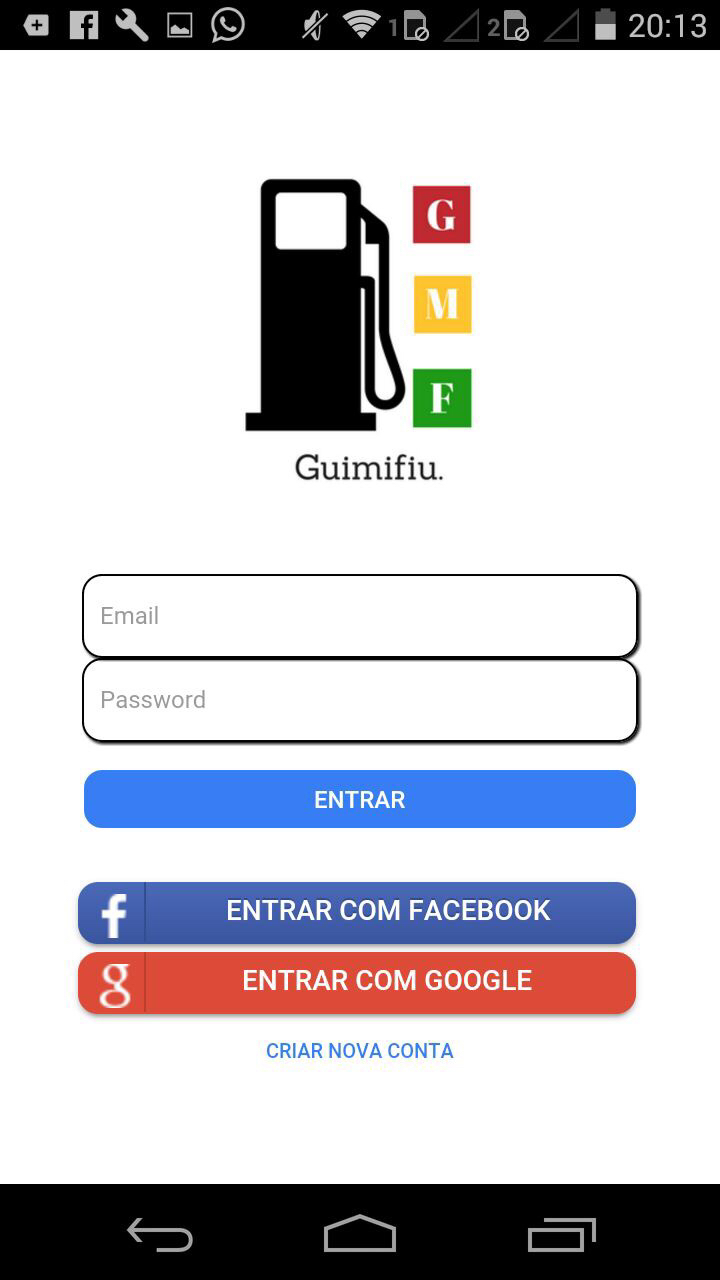
\includegraphics[scale=0.2]{figuras/app_1.jpg}
    \caption[Tela de login]{Tela de login. Fonte: autores}
    \label{img:tela_de_login}
\end{figure}
\pagebreak

Como ilustrado na Figura \ref{img:postos_de_gasolina_proximos}, são mostrados na aplicação todos os postos de com- bustíveis em um raio de 5 km da localização do usuário.

\begin{figure}[H]
    \centering
    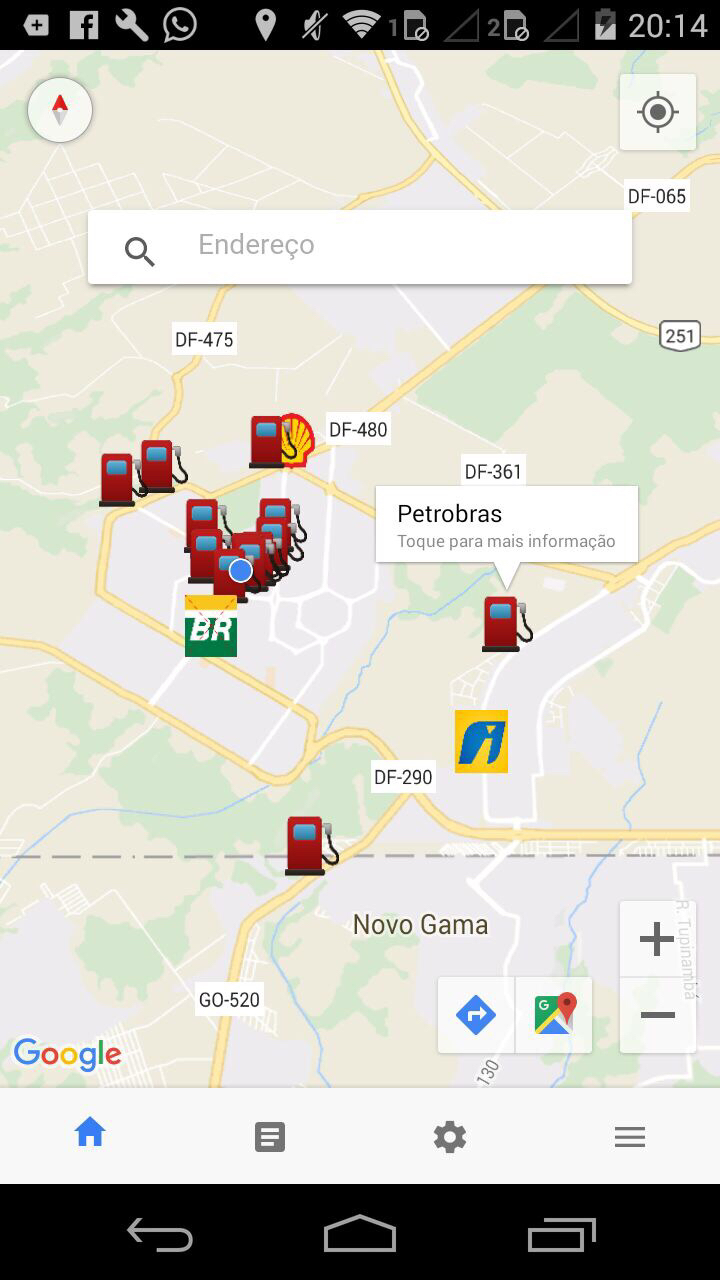
\includegraphics[scale=0.2]{figuras/app_2.jpg}
    \caption[Postos de combustíveis próximos]{Postos de combustíveis próximos à localização do usuário. Fonte: autores}
    \label{img:postos_de_gasolina_proximos}
\end{figure}

A Figura \ref{img:chegou-posto-boicotado} mostra uma tela da aplicação assim que se chega em um posto boicotado.

\begin{figure}[H]
    \centering
    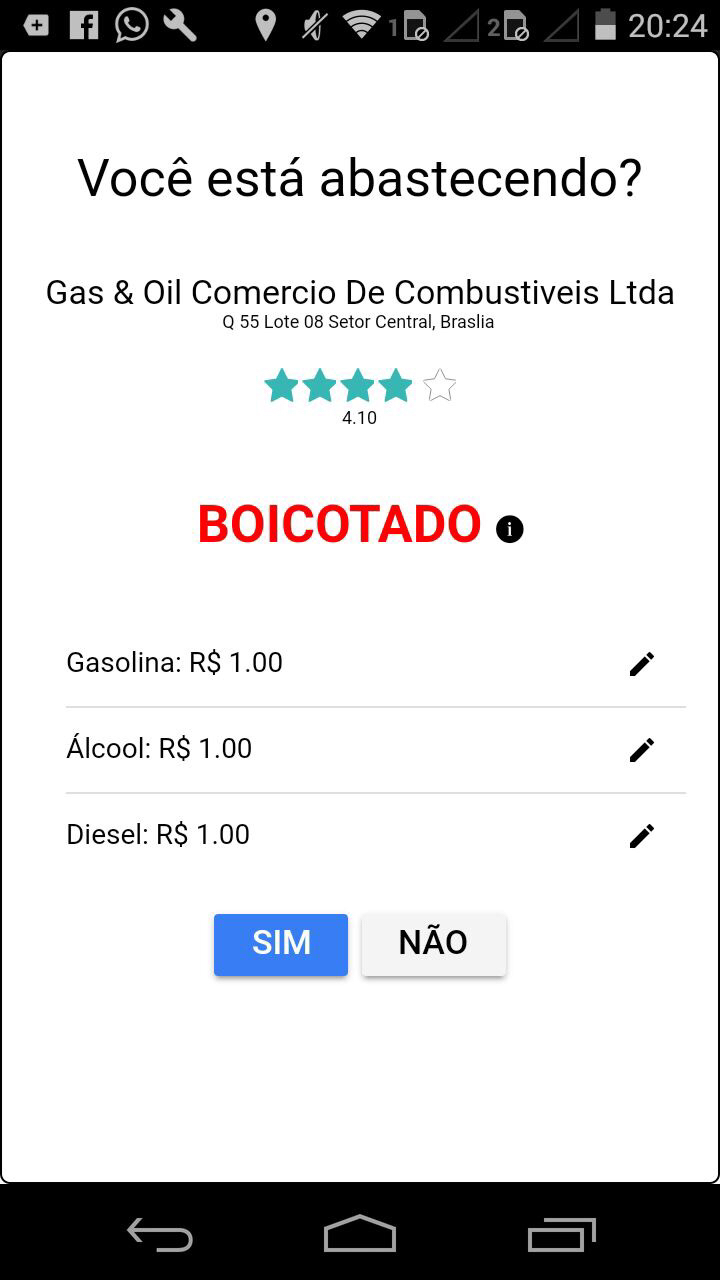
\includegraphics[scale=0.2]{figuras/chegou-posto.jpg}
    \caption[Tela de chegada no posto boicotado]{Tela de chegada no posto boicotado. Fonte: autores}
    \label{img:chegou-posto-boicotado}
\end{figure}

Além desses requisitos, foram elicitados as novas histórias que se mostraram imprescindíveis para a aplicação. O status dos requisitos se encontram na Tabela \ref{tab:req-2}

\begin{table}[H]
\centering
\caption{Status dos Requisitos elicitados na segunda entrega}
\label{tab:req-2}
\begin{tabular}{|c|c|}
\hline
\textbf{História} & \textbf{Desenvolvida?} \\ \hline
15                & Sim                    \\ \hline
16                & Sim                    \\ \hline
17                & Sim                    \\ \hline
18                & Sim                    \\ \hline
19                & Sim                    \\ \hline
20                & Sim                    \\ \hline
21                & Sim                    \\ \hline
\end{tabular}
\end{table}

As funcionalidades de administrador se mostraram imprescindíveis para facilitar a identificação dos postos de combustíveis pelo usuário através de ícones, indicando as bandeiras. Durante o segundo período do projeto, observou-se que algumas informações fornecidas pela API do Google possuíam erros. Com o módulo de administração, é possível corrigir esses erros pontuais. Além disso, como a primeira versão do aplicativo que vai para a Play Store não possuirá as funcionalidades que garantirão a qualidade dos dados de preços dos combustíveis, a possibilidade de editar os dados de sugestão de preço manualmente, de forma mais prática, mostrou-se importante. A Figura \ref{img:admin-1} mostra a página inicial do módulo de administração.

\begin{figure}[H]
    \centering
    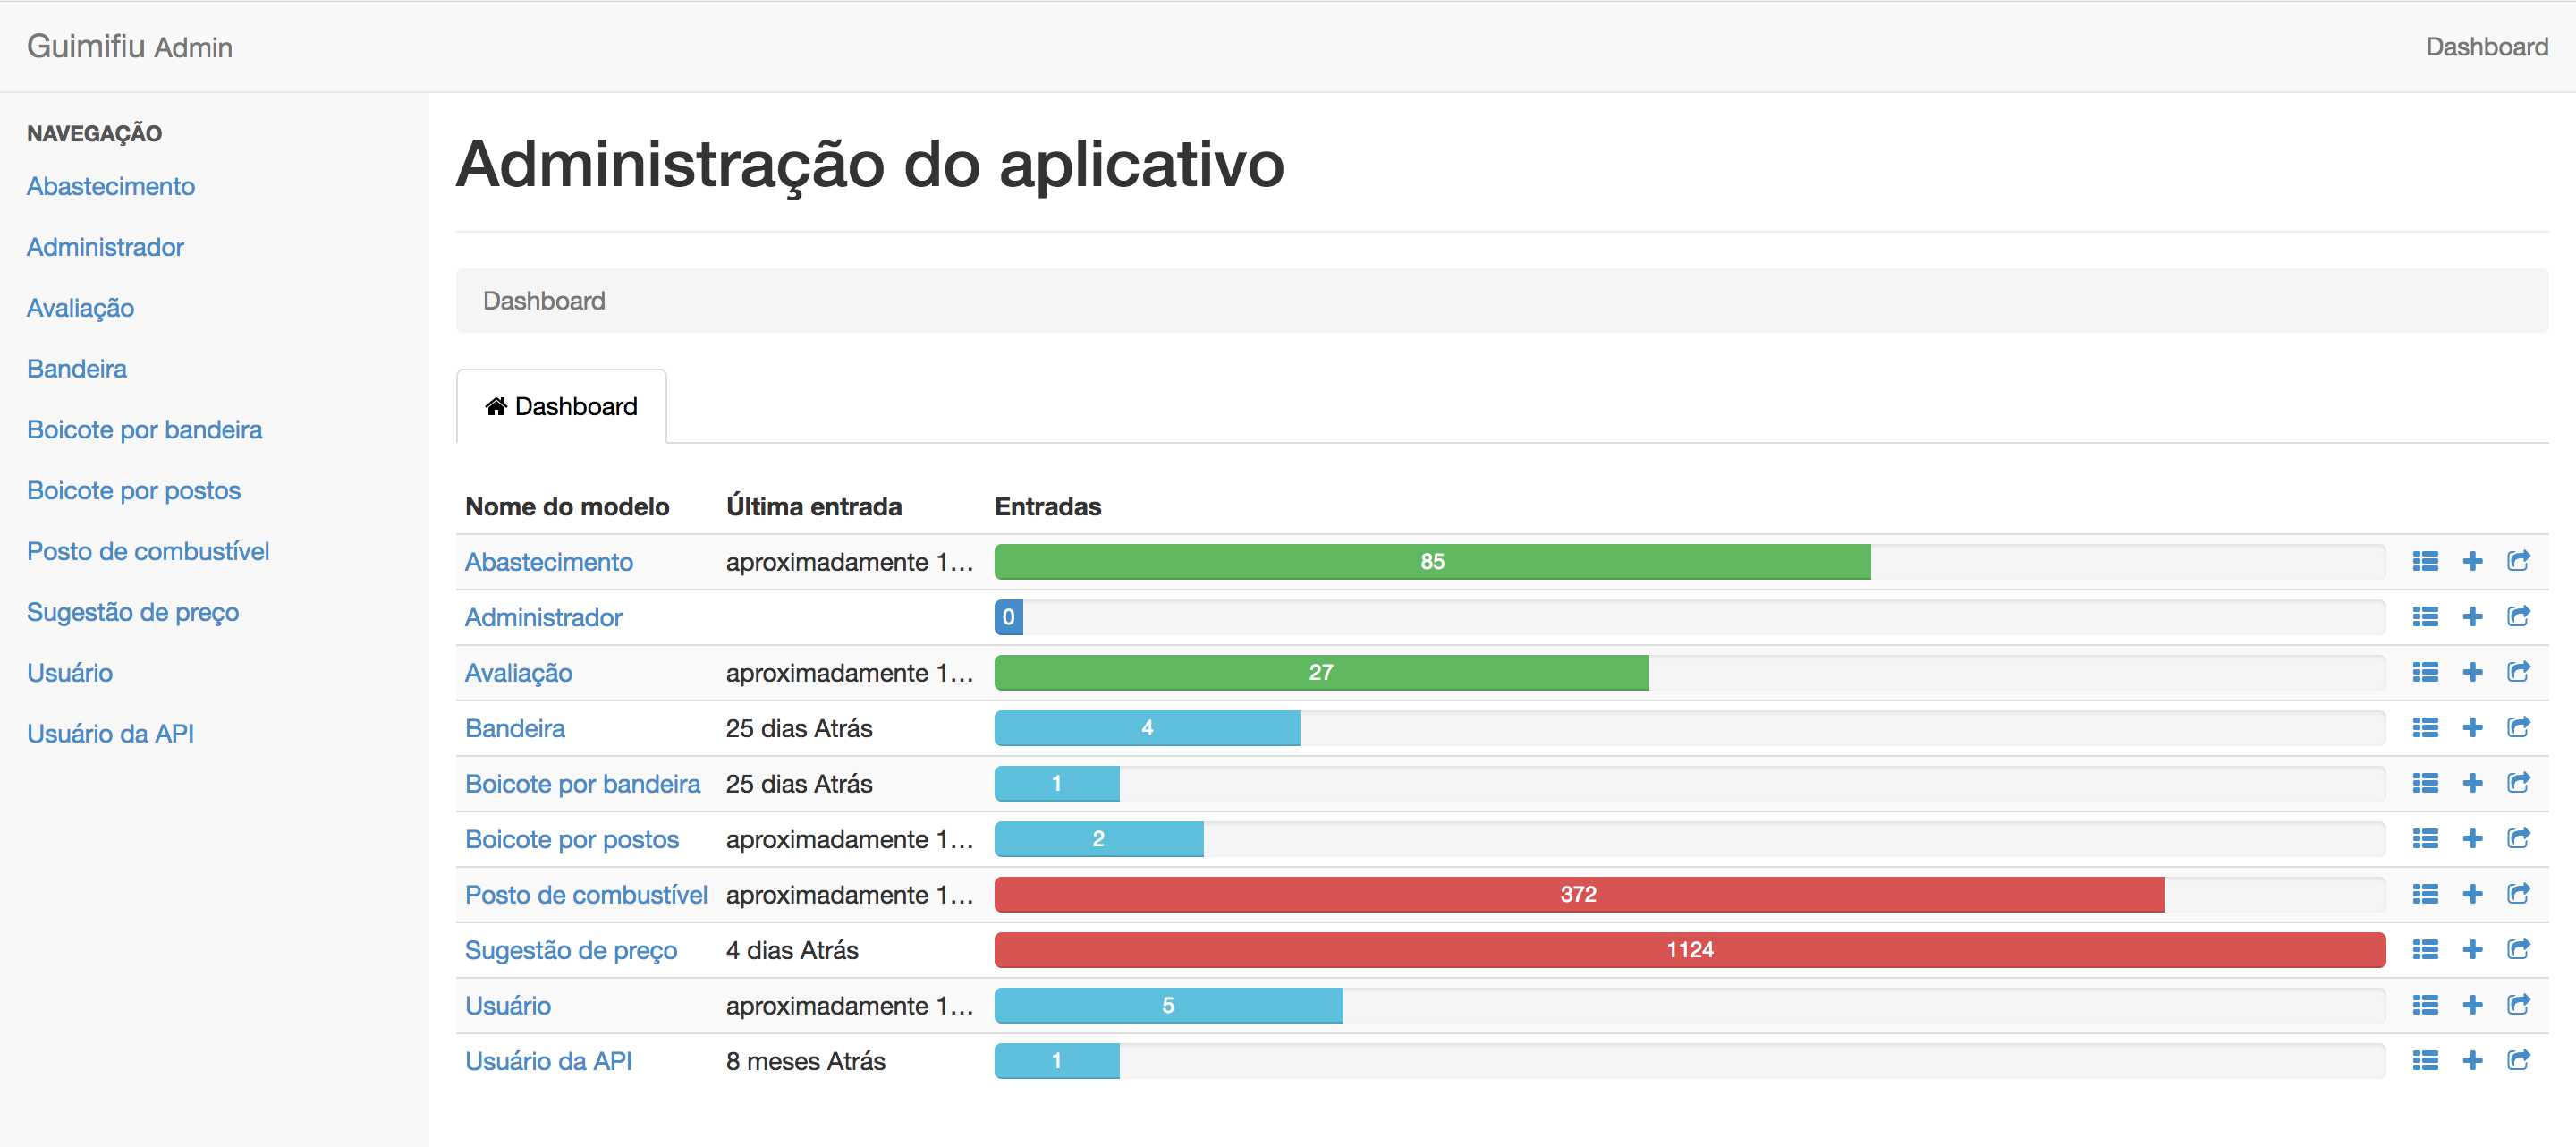
\includegraphics[scale=0.32]{figuras/admin-1.png}
    \caption[Página inicial do módulo de administração]{Página inicial do módulo de administração. Fonte: autores}
    \label{img:admin-1}
\end{figure}

Observou-se também a importância de manter um controle na aplicação sobre o controle de gastos do motorista e como essa funcionalidade é um diferencial em relação aos aplicativos atuais. A Figura \ref{img:historico-app} ilustra o histórico de postos abastecidos pelo usuário, enquanto a Figura \ref{img:grafico-app} mostra o gráfico de gastos mensais.

\begin{figure}[H]
    \centering
    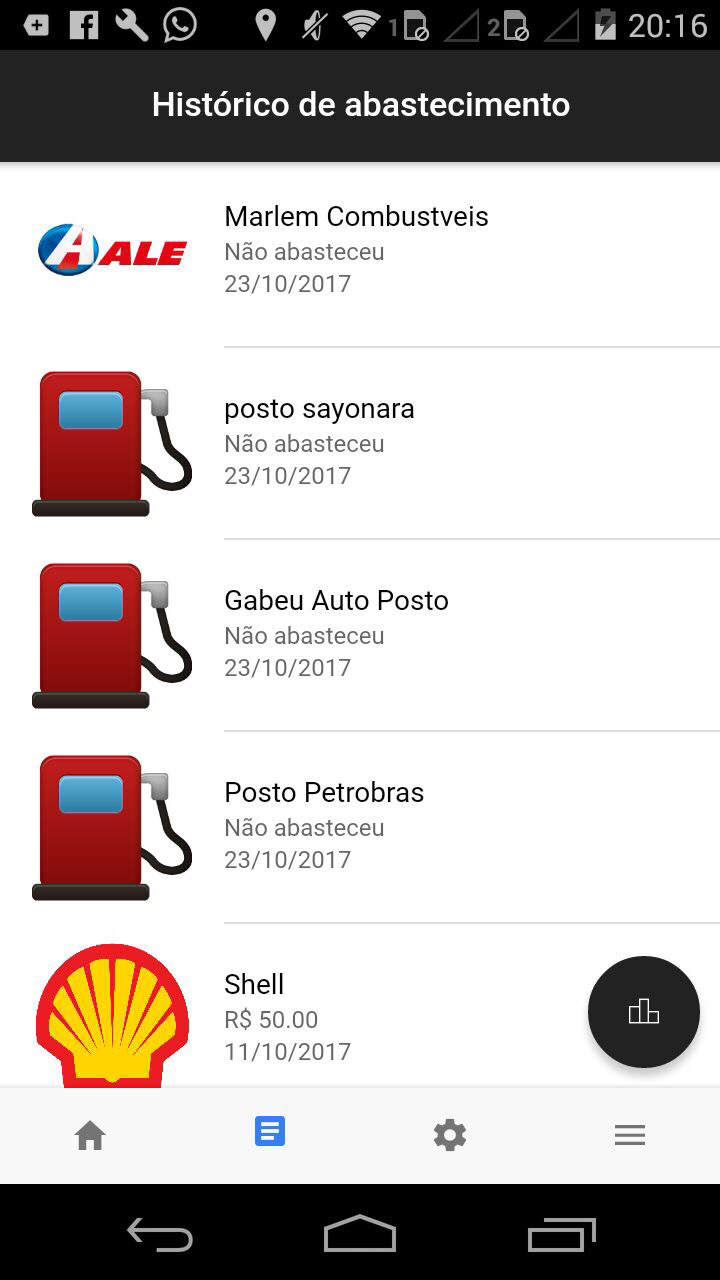
\includegraphics[scale=0.2]{figuras/historico-app.jpg}
    \caption[Página inicial do módulo de administração]{Página inicial do módulo de administração. Fonte: autores}
    \label{img:historico-app}
\end{figure}

\begin{figure}[H]
    \centering
    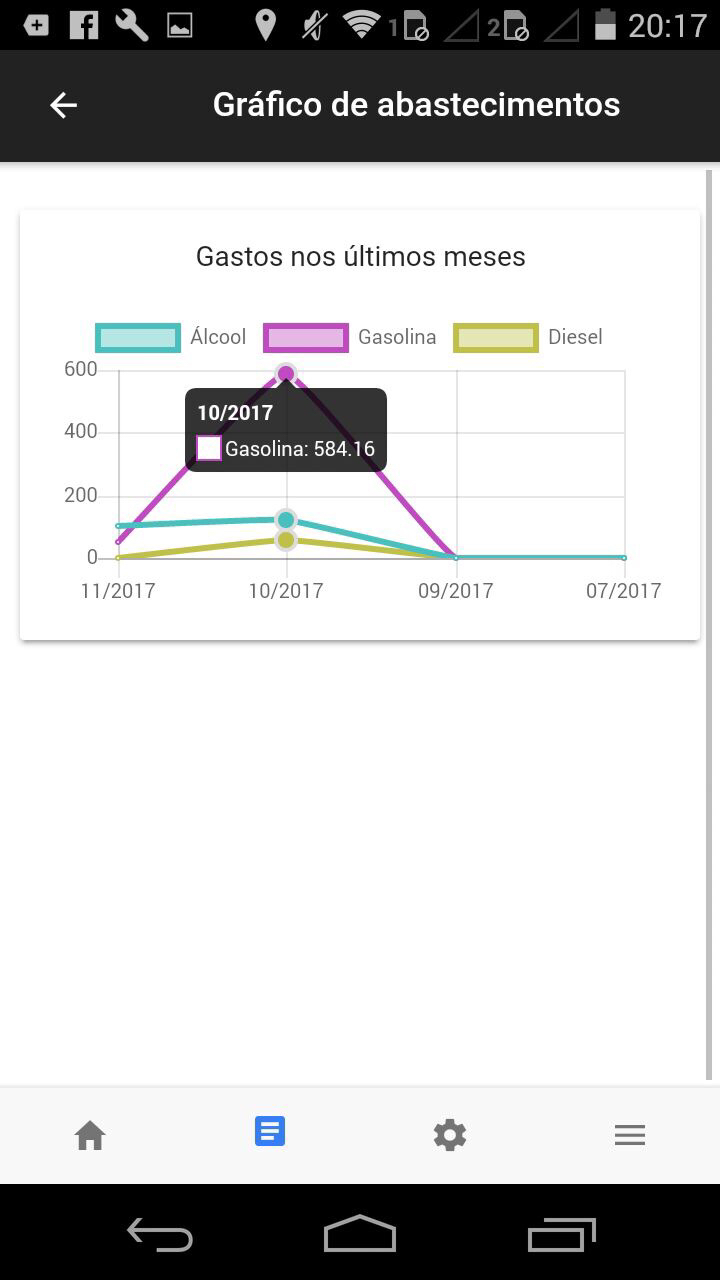
\includegraphics[scale=0.2]{figuras/grafico-app.jpg}
    \caption[Página inicial do módulo de administração]{Página inicial do módulo de administração. Fonte: autores}
    \label{img:grafico-app}
\end{figure}
\pagebreak

Com as funcionalidades implementadas, a comunicação dos sistemas desenvolvidos se dá como ilustrado pela Figura \ref{img:comunicacaosistemas}:

\begin{figure}[H]
    \centering
    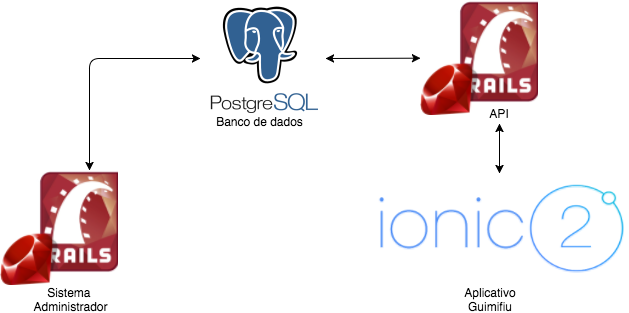
\includegraphics[scale=0.5]{figuras/comunicacao_sistemas.png}
    \caption[Comunicação entre os sistemas desenvolvidos.]{Comunicação entre os sistemas desenvolvidos. Fonte: autores}
    \label{img:comunicacaosistemas}
\end{figure}

Os dados armazenados em um banco de dados PostgreSQL são transacionados pela interface administradora e pela API. Por sua vez, aplicativo se comunica com a API para acessar, criar e alterar os dados.

O Apêndice \ref{chap:telas} apresenta algumas outras telas da aplicação desenvolvida.

\subsection{Método de decisão de postos boicotados}
Toda semana, serão selecionados postos onde os usuários serão incentivados a não abastecer. Para decidir quais postos serão boicotados, o Guimifiu tem duas estratégias principais: a \textbf{Lista Comum} e o \textbf{Boicote por Bandeiras}. A lista comum escolhe os postos com qualidade geral menor que 1 e que não tenham sido boicotados recentemente, criando uma lista inicial. A qualidade geral de um posto é determinada pela fórmula a seguir, onde são considerados o número de estrelas do posto e o preço dos combustíveis:

\begin{equation}
\label{Equação para cálculo de qualidade geral do Combustível}
	QG = \frac{5*QE}{2*(PG + PA + PD)}
\end{equation}

Sendo que QG é a Qualidade Geral do posto, PG, PA e PD são os preços de Gasolina, Álcool e Diesel, respectivamente e, por fim, QE é a Quantidade de Estrelas. A quantidade de estrelas é definida pela média das avaliações dos usuários. O objetivo é que a qualidade do posto indicado pelos usuários seja proporcional à qualidade geral dele e que os preços dos combustíveis sejam inversamente proporcionais, ou seja, quanto maior a quantidade de estrelas e menor o preço dos combustíveis, maior a qualidade geral do posto, diminuindo suas chances do mesmo ser boicotado. Essa fórmula será balanceada de acordo com os dados dos postos e das avaliações dos usuários com o tempo. A tabela \ref{tab:exemplo} contém um exemplo de postos fictícios com preços, quantidade de estrelas e a qualidade geral.

\begin{table}[H]
\centering
\caption{Tabela de postos fictícios}
\label{tab:exemplo}
\begin{tabular}{|c|c|c|c|c|c|}\hline
\textbf{Posto} & \textbf{PG}   & \textbf{PA}   & \textbf{PD}   & \textbf{QE}  & \textbf{QG}   \\
\hline
1     & 4,00 & 3,00 & 4,00 & 2   & 0,45 \\ \hline
2     & 3,90 & 3,20 & 4,50 & 5   & 1,07 \\ \hline
3     & 4,00 & 3,50 & 3,70 & 4,5 & 1,00 \\ \hline
4     & 4,00 & 3,80 & 3,90 & 3,5 & 0,74 \\ \hline
5     & 4,00 & 3,80 & 3,90 & 4,5 & 0,96 \\ \hline
\end{tabular}
\end{table}

Na tabela \ref{tab:exemplo}, os postos 1, 4 e 5 seriam os colocados na lista inicial, devido ao baixo QG. Os postos 2 e 3 estariam logo acima do limite mínimo e, portanto, estariam de fora da lista.

A lista inicial é montada e então a aplicação verifica se não existem muitos postos próximos sendo boicotados, para não deixar o usuário com poucas opções de locais de abastecimento. Essa verificação é feita através de grafos. Os nós dos grafos são os postos de combustíveis e as arestas são as distâncias entre os todos postos que não sejam maiores que 10 quilômetros. Com este grafo, em cada nó da lista inicial é verificado se os nós adjacentes são todos postos que estão na lista inicial. Em caso positivo, o nó é removido da lista; caso contrário, o nó é mantido. Os nós restantes compõem a lista final de postos boicotados, denominada \textbf{Lista Comum}. Na Figura \ref{img:listainicial}, considerando que os pontos vermelhos são nós da lista inicial e os pontos azuis são os demais postos, após a verificação, os pontos vermelhos virariam azuis, como mostrado na Figura \ref{img:listacomum}.

\begin{figure}[H]
    \centering
    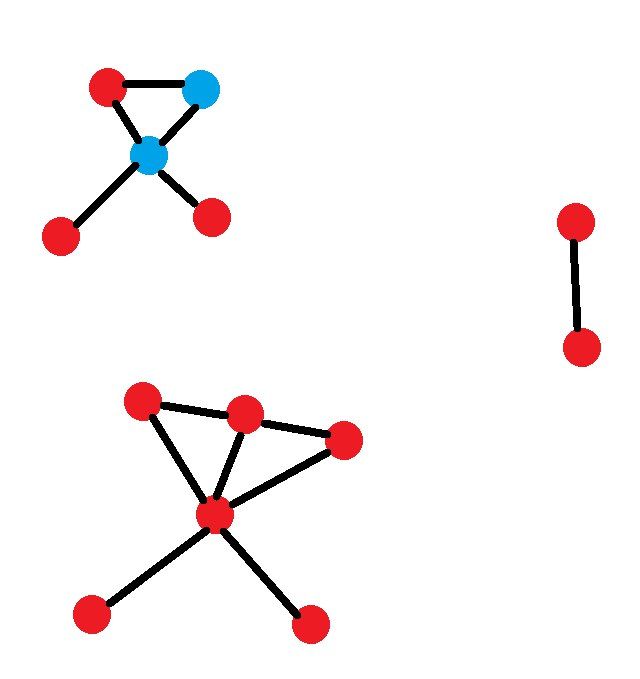
\includegraphics[scale=0.4]{figuras/listainicial.jpg}
    \caption[Grafo com Lista Inicial de Postos Boicotados]{Grafo com Lista Inicial de Postos Boicotados. Fonte: autores}
    \label{img:listainicial}
\end{figure}

\begin{figure}[H]
    \centering
    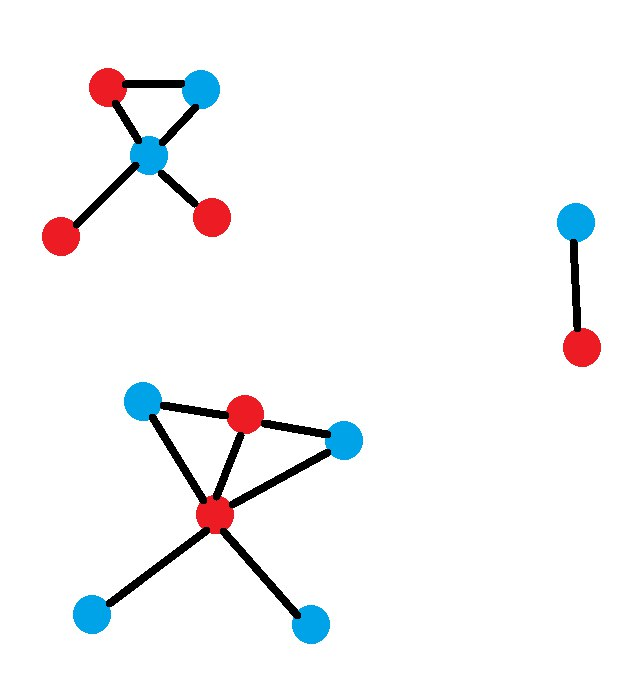
\includegraphics[scale=0.4]{figuras/listacomum.jpg}
    \caption[Grafo com Lista Comum de Postos Boicotados]{Grafo com Lista Comum de Postos Boicotados. Fonte: autores}
    \label{img:listacomum}
\end{figure}

Baseado no algoritmo, foi desenvolvido um script na linguagem Ruby que é executado semanalmente no servidor hospedado no Heroku, através do \textit{Heroku Scheduler}, uma ferramenta criada para executar tarefas no servidor.

O \textbf{Boicote por Bandeiras} acontece quando todos os postos de uma bandeira previamente selecionada são colocados na lista de boicotados, independentemente da distância entre eles, colocando o prejuízo do boicote menos nos postos e mais na bandeira. Os dois tipos de boicote são exclusivos, ou seja, não ocorrem no mesmo período. A estratégia de boicote é escolhida pela equipe de desenvolvimento. O \textbf{Boicote por Bandeiras} é iniciado manualmente no módulo de administração, como mostra a Figura \ref{img:admin-2}

\begin{figure}[H]
    \centering
    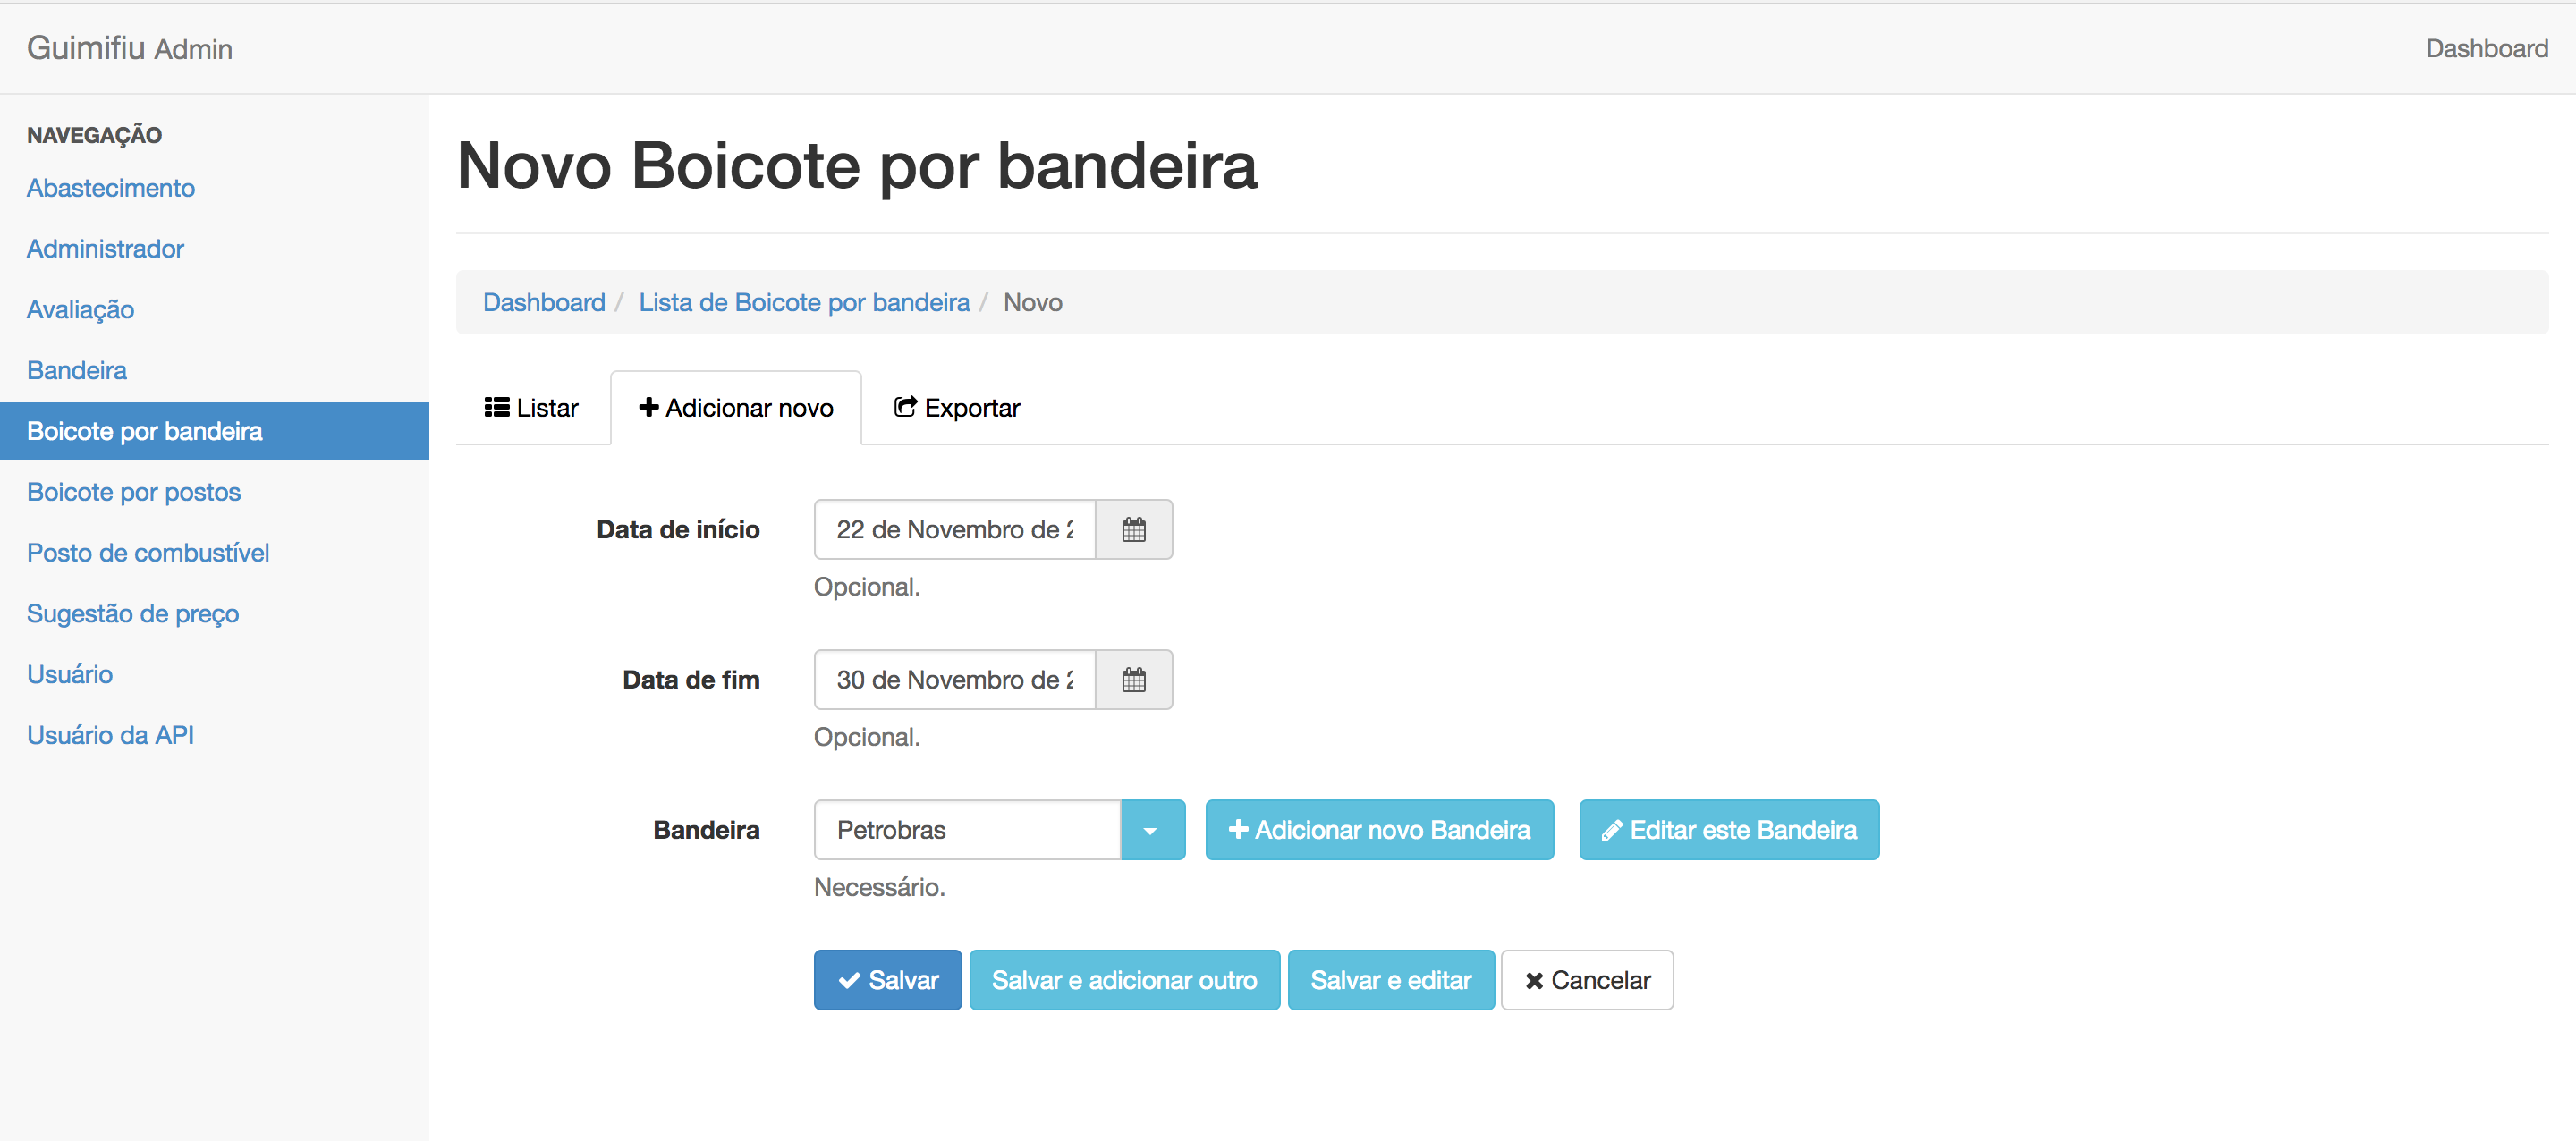
\includegraphics[scale=0.32]{figuras/admin-2.png}
    \caption[Página de criação de Boicotes do módulo de administração]{Página de criação de Boicotes do módulo de administração. Fonte: autores}
    \label{img:admin-2}
\end{figure}

\subsection{Testes Automatizados}

Foram feitos testes de integração e unitários para garantir o funcionamento dos métodos do código-fonte e da integração da aplicação \textit{mobile} com a API.

Encontrou-se uma certa dificuldade pra realizar os testes unitários no Ionic, uma vez que não há muitos exemplos que de fato funcionam e uma documentação do próprio \textit{framework} sobre o assunto.

O código de testes pode ser encontrado no repositório da aplicação no GitHub (https://github.com/Guimifiu/guimifiu-app). Um exemplo de teste unitário e de teste de integração está disponível no Apêndice \ref{chap:testes}.

\subsection{Métricas de Código-fonte}

Como citado no \autoref{chap:met}, foram utilizadas as ferramentas CodeClimate e Rubocop. Além de medir a complexidade no Rubocop, foi feita na integração contínua um relatório de métricas pela ferramenta que impede que a \textit{build} passe caso a complexidade seja maior do que 6, que é o padrão de complexidade ciclomática máxima aceitável.

A Figura \ref{img:rubocop} mostra o resultado da análise feita pelo Rubocop. O arquivo de configuração utilizado para a análise pode ser encontrado no endereço do GitHub do  \citeonline{rubocop-guimifiu}.

\begin{figure}[H]
    \centering
    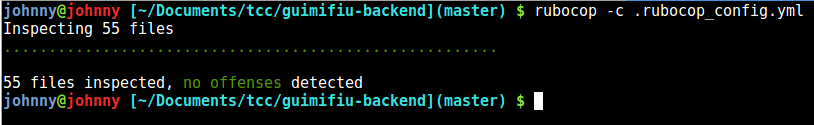
\includegraphics[scale=0.5]{figuras/rubocop.png}
    \caption[Relatório de análise estática do Rubocop]{Relatório de análise estática do Rubocop. Fonte: autores}
    \label{img:rubocop}
\end{figure}

A Figura \ref{img:codeclimate} mostra o resultado das análises realizado pelo \href{https://codeclimate.com/github/Guimifiu/guimifiu-backend/}{CodeClimate}.

\begin{figure}[H]
    \centering
    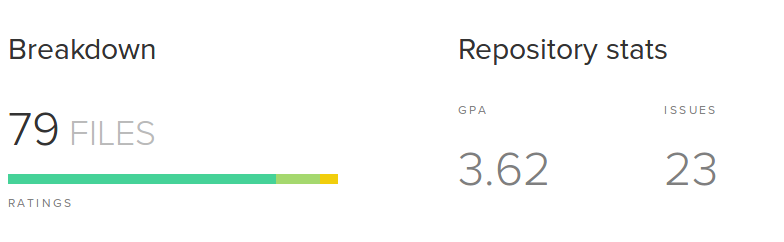
\includegraphics[scale=0.5]{figuras/codeclimate.png}
    \caption[Relatório de análise estática do CodeClimate]{Relatório de análise estática do CodeClimate. Fonte: autores}
    \label{img:codeclimate}
\end{figure}

As \textit{issues} encontradas no CodeClimate infelizmente não puderam ser tratadas a tempo da entrega do projeto devido aos problemas encontrados durante o desenvolvimento, como descritos no Capítulo \ref{chap:crono}.


\subsection{Integração e Entrega Contínua}
Há três tipos de ambientes no desenvolvimento desta aplicação: \textit{development}, \textit{staging} e \textit{production}. O ambiente de \textit{development} ou desenvolvimento, é o ambiente local de cada desenvolvedor, \textit{staging} ou pré produção é um ambiente para serem realizados testes beta e \textit{production} ou produção é o ambiente final onde a aplicação será de fato utilizada pelos usuários.

Na API a integração contínua é feita com a ferramenta TravisCI. Onde, se um \textit{pull request} é aceito na \textit{branch} \textit{staging}, o Travis executa toda a suíte de testes para ver se algum deles pode ter resultado em falha, caso todos passem, ele verifica se todas as métricas definidas pelo Rubocop estão de acordo com o padrão definido. Caso todas as métricas passem, a build de pré produção é criada, o Travis envia as informações de cobertura de testes para o Coveralls, as informações de métricas para o Code Climate e logo em seguida realiza o \textit{deploy} no ambiente de pré produção no Heroku.

Caso um \textit{pull request} seja aceito na \textit{branch} \textit{master} todo o processo será o mesmo, com exceção que o \textit{deploy} irá ocorrer no ambiente de produção no Heroku.

A figura \ref{img:integracao_deploy_continuo_api} ilustra o processo de integração e deploy contínuo feito na API.

\begin{figure}[H]
    \centering
    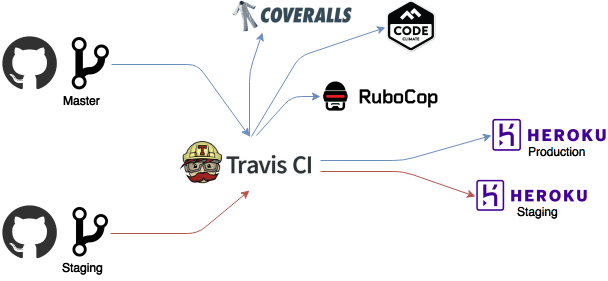
\includegraphics[scale=0.5]{figuras/api_ci.png}
    \caption[Integração e deploy contínuo API]{Integração e deploy contínuo API.}
    \label{img:integracao_deploy_continuo_api}
\end{figure}

No aplicativo, foi planejada a integração e o deploy contínuo para ocorrer da seguinte forma:

\begin{figure}[H]
    \centering
    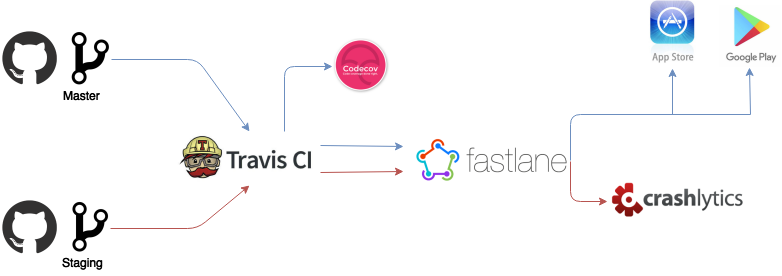
\includegraphics[scale=0.5]{figuras/ci_should_be.png}
    \caption[Integração e deploy contínuo planejado para o APP]{Integração e deploy contínuo planejado para o APP}
    \label{img:integracao_deploy_continuo_planejado_app}
\end{figure}

Se um pull request \textit{pull request} é aceito na \textit{branch} \textit{master}, o Travis irá realizar toda a suíte de testes, caso todos passem enviará as informações de cobertura para o
Codecov e através do Fastlane realizará o deploy do aplicativo tanto na Play Store quanto na App Store. E caso um \textit{pull request} é aceito na \textit{branch} \textit{staging}, todo o processo é repetido, com exceção
que não é realizado o deploy do aplicativo nas lojas e sim no Crashlytics, que irá criar a versão beta do aplicativo e enviará por email para os emails configurados previamente.

Uma vez que o aplicativo ainda não chegou ao estágio de deploy nas lojas, o planejamento para a primeira entrega é só até o deploy beta, como mostrado na figura \ref{img:integracao_deploy_continuo_planejado_primeira_entrega}:

\begin{figure}[H]
    \centering
    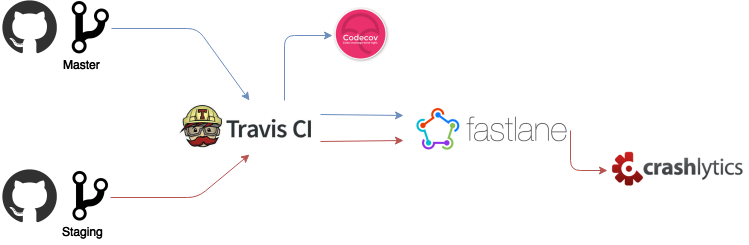
\includegraphics[scale=0.5]{figuras/ci_as_is.png}
    \caption[Integração e deploy contínuo planejado para o APP]{Integração e deploy contínuo planejado para a primeira entrega}
    \label{img:integracao_deploy_continuo_planejado_primeira_entrega}
\end{figure}

Porém não foi possível fazer com que o deploy contínuo aconteça logo após a integração contínua, um desafio causado por escolher desenvolvimento híbridos de aplicativo.
Uma vez que o código versionado do aplicativo é o mesmo código para a plataforma Android e iOS, e após realizar a build desse código é gerado códigos em cada plataforma (não versionados),
a ferramenta de integração contínua não consegue ter acesso aos códigos de cada plataforma para realizar os devidos deploys. Sendo assim, o deploy contínuo está acontecendo manualmente
por enquanto que nenhuma solução ainda foi encontrada, através do comando:

\begin{lstlisting}[language=bash]
  $ fastlane beta
\end{lstlisting}

Sendo assim, a figura \ref{img:integracao_deploy_continuo_atual} ilustra como está funcionando a integração e o deploy contínuo do aplicativo até o presente momento.

\begin{figure}[H]
    \centering
    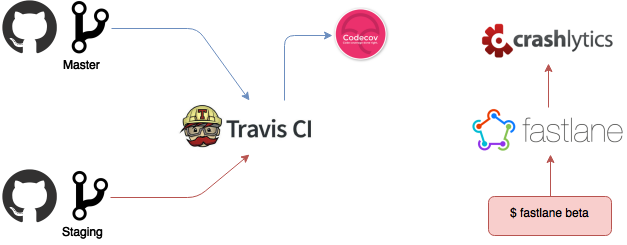
\includegraphics[scale=0.5]{figuras/ci_currently.png}
    \caption[Integração e deploy contínuo atual]{Integração e deploy contínuo atual}
    \label{img:integracao_deploy_continuo_atual}
\end{figure}

